% Lecture Template for ME3023 -  Measurements in Mechanical Systems - Tennessee Technological University
% Spring 2020 - Summer 2020 - Fall 2020 - Spring 2021 - Summer 2021
% Tristan Hill, May 07, 2020 - June 12, 2020 - July 08, 2020 - Novemeber 02, 2020 - March 28, 2021 - May 25, 2021
% Module Name: To Err is Human
% Topic 2 - Errors and Uncertainty

\documentclass[fleqn]{beamer} % for presentation (has nav buttons at bottom)
\usepackage{../../measurements_lectures}

\author{ME3023 - Measurements in Mechanical Systems} 

%\newcommand{\MNUM}{2\hspace{2mm}} % Module number
\newcommand{\TNUM}{2\hspace{2mm}} % Topic number 
\newcommand{\moduletitle}{To Err is Human}
\newcommand{\topictitle}{Errors and Uncertainty} 

\newcommand{\sectiontitleI}{Random and Systematic Errors}
\newcommand{\sectiontitleII}{Dart Board Example}
\newcommand{\sectiontitleIII}{Types of Errors}
\newcommand{\sectiontitleIV}{Sample Uncertainty Data}

\setbeamercolor{title in head/foot}{fg=TTUgold} % this needs work...

% custom box
\newsavebox{\mybox}

\title{Lecture Module - \moduletitle}

\date{Mechanical Engineering\vspc Tennessee Technological University}

\begin{document}
	
	\lstset{language=MATLAB,basicstyle=\ttfamily\small,showstringspaces=false}
	
	\frame{\titlepage \center\begin{framed}\Large \textbf{Topic \TNUM - \topictitle}\end{framed} \vspace{5mm}}

% Section 0: Outline
\begin{frame}

\large \textbf{Topic \TNUM - \topictitle} \vspace{3mm}\\

\begin{itemize}

	\item \hyperlink{sectionI}{\sectiontitleI} \vspc % Section I
	\item \hyperlink{sectionII}{\sectiontitleII} \vspc % Section II
	\item \hyperlink{sectionIII}{\sectiontitleIII} \vspc %Section III
	\item \hyperlink{sectionIV}{\sectiontitleIV} \vspc %Section IV

\end{itemize}

\end{frame}

% Section 1
\section{\sectiontitleI}

\begin{frame}[label=sectionII]
\frametitle{\sectiontitleI}

"Errors are effects that cause a  measured value to differ from its true value. \hspcu error causes a
\hspcu variation in measured values found during repeated measurements of a variable. \vspc
\hspcu error causes an offset between the mean value of the data set and its true value. Both \hspcu and
\hspcu errors affect a system's accuracy."

\vspace{10mm}
{\tiny Text: Theory and Design of Mech. Meas.}
\end{frame}

% Section 2
\section{\sectiontitleII}

\begin{frame}[label=sectionIII]
\frametitle{\sectiontitleII}

"The concept of accuracy and the effects of \hspcu and \hspcu errors in instruments
and measurement systems can be illustrated by the throw of darts."

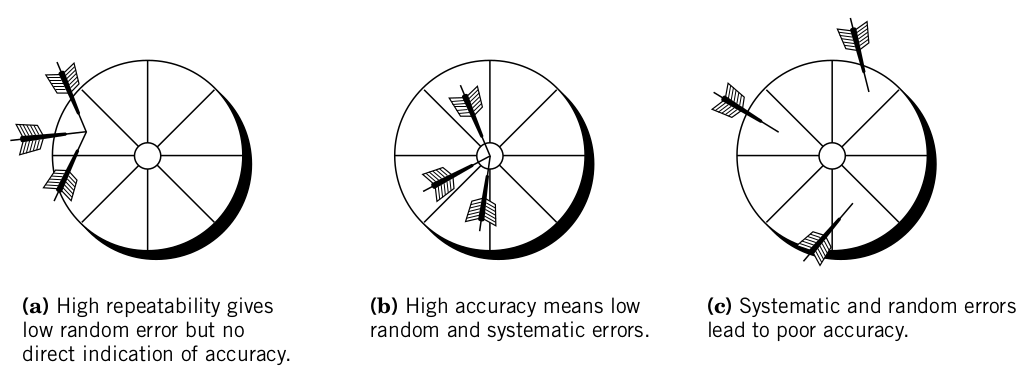
\includegraphics[scale=.20]{dart_throw.png}

The ability of a measurement system to indicate the same value on repeated but independent
application of the same input provides a measure of the instrument \hspcu."

{\tiny Text, Image: Theory and Design of Mech. Meas.}
\end{frame}


% Section 3
\section{\sectiontitleIII}

\begin{frame}[label=sectionIII]
\frametitle{\sectiontitleIII}

Common categories of errors in measurements are shown below. This is not an exhaustive list.  

\begin{itemize}
	
	\item Linearity Error \vspc
	\item Sensitivity \vspc
	\item Zero (offset) Error \vspc
	\item Hysteresis Error \vspc
	\item Overall Instrument Error \vspc
\end{itemize}

\scalebox{1}{$u_c=\sqrt{u_1^2+u_2^2+...+u_M^2}$}

\end{frame}

% Section 4
\section{\sectiontitleIV}

\begin{frame}[label=sectionIV]
\frametitle{Sample Uncertainty Data}

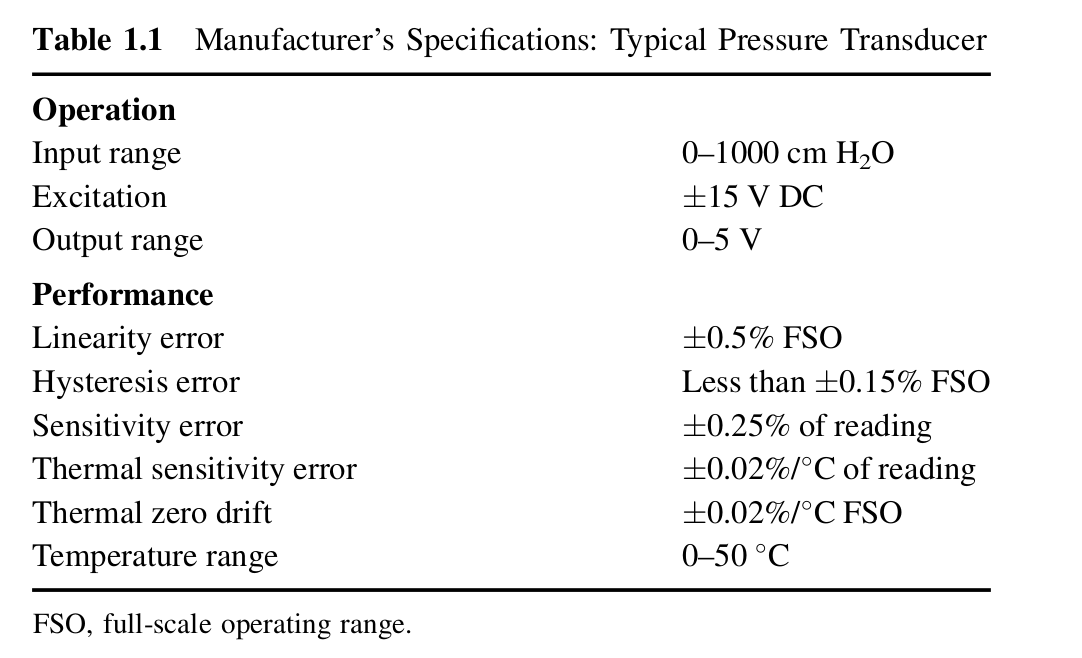
\includegraphics[scale=.22]{sample_uncertainties.png}

{\tiny Text, Image, Data: Theory and Design of Mech. Meas.}

\end{frame}

\end{document}





